\chapter{علم الجراثيم: النمو والفيزيولوجيا والوراثة}\label{ch:b3:bacteriology}

خلية واحدة من \emph{Escherichia coli} في مرق دافئ تنقسم كل
عشرين دقيقة. ولو تُركت من غير كابح لفاقت ذريتها الأرضَ
وزنًا في يومين؛ لكنها تتوقف في الواقع في ساعات، حين ينفد السكر،
وتقعد أسابيع في حالة تنجو من الجوع. وبكتيريا
قريبة، إذا أُعطيت جرحًا وبضع ساعات، تصير مئة مليون
خلية وحمّى؛ وقبل مئة سنة كانت تقتل ثلث
المرضى الذين تخمجهم، ومنذ عام 1941 أنقذ سمّ عفن ضدها
أرواحًا أكثر من أي دواء آخر --- بينما طوّرت البكتيريا، على مدى
الثمانين سنة نفسها، سبلًا للالتفاف على كل \omterm{def:b3:bacteriology:antibiotics}{مضاد حيوي} صُنع.
وقد كانت البكتيريا الكائنات التي بُيّن فيها أول مرة أن المورّثات
DNA، وفُهم فيها التنظيم المورّثي أول مرة، ومنها أُخذت
أدوات \cref{ch:b3:genetic-engineering}. ويتناولها هذا الفصل
بوصفها كائنات: غلافها، وحساب نموها في دورق وفي
مزرعة مستمرة، وكيف تستشعر جمهرتها كثافتها هي،
وحركة المورّثات بين الخلايا، وكيمياء المضادات الحيوية والمقاومة وتطورها.

\section{الخلية البكتيرية}

\begin{definition}[الغلاف]\label{def:b3:bacteriology:envelope}
\index{ببتيدوغليكان}\index{إيجابي الغرام}\index{سلبي الغرام}\index{غشاء خارجي}\index{عديد سكريد شحمي}\index{بوغ داخلي}
كل بكتيريا إلا قليلًا محاطة بجدار من \emph{الببتيدوغليكان}:
سلاسل من N-أستيل غلوكوزامين وحمض N-أستيل موراميك بالتناوب،
مشبَّكة بببتيدات قصيرة في جزيء واحد يحيط
بالخلية ويقاوم ضغط الامتلاء --- وهو عدة جوّات ---
في الهيولى. والبكتيريا \emph{إيجابية الغرام} لها جدار ثخين من
\qtyrange{20}{80}{nm}، بطبقات كثيرة، تتخلله حموض التيكويك؛
والبكتيريا \emph{سلبية الغرام} لها جدار رقيق من طبقة أو طبقتين
وخارجه طبقة دهنية ثنائية ثانية هي \emph{الغشاء الخارجي}،
ووريقته الخارجية \emph{عديد سكريد شحمي} (LPS، وهو الذيفان الداخلي ---
الجزيء الذي تتعرفه المناعة الفطرية في
\cref{ch:b3:innate-immunity} والذي يسبب الصدمة الإنتانية)،
محيطًا بالمحيط حول البلازما. والبورينات في الغشاء الخارجي تُدخل الجزيئات
الصغيرة وتستبعد كثيرًا من المضادات الحيوية. وقد تقع في الخارج محفظة من
عديد السكريد تقي من البلعميات، وأسواط للسباحة
(\cref{ch:b3:cytoskeleton-motility})، وأهلاب للالتصاق و
\omterm{def:b3:bacteriology:hgt}{الاقتران}. وفي الداخل يُطوى الصبغي --- وهو جزيء حلقي واحد من
\qtyrange{1}{10}{Mb} في معظم الأنواع --- في نُوَيد
بلا غشاء، بجانب البلازميدات. وبعض الأجناس (\emph{Bacillus}، و
\emph{Clostridium}) يستطيع أن يحبس نسخة من الصبغي في غلاف
ثخين بوغًا \emph{داخليًا}، مجففًا خامل الاستقلاب، ينجو
من الغليان والإشعاع وقرون من الجفاف وينبت
حين تعود المغذيات.
\end{definition}

\begin{method}[صبغة غرام]\label{met:b3:bacteriology:gram}
\index{صبغة غرام}
أقدم اختبار في مختبر الجراثيم (غرام، 1884) ما يزال
يقرر أول اختيار \omterm{def:b3:bacteriology:antibiotics}{لمضاد حيوي}. (1) الطخ العينة وثبّتها بالحرارة؛
(2) اصبغ بالبنفسجي البلوري، ثم باليود، الذي يكوّن
معقّدًا كبيرًا غير ذواب مع الصبغ داخل الخلايا؛ (3) اغسل
بالكحول: \omterm{def:b3:bacteriology:envelope}{فالببتيدوغليكان} الثخين في إيجابيات الغرام، وقد جففه
الكحول، يحبس المعقّد فتبقى الخلايا بنفسجية، بينما يدع الجدار الرقيق
في سلبيات الغرام المعقّدَ يخرج؛ (4) اصبغ صبغة مضادة بالسافرانين،
التي تلوّن سلبيات الغرام، وقد صارت عديمة اللون، بالوردي. والشكل
والترتيب --- مكورات في عناقيد (عنقوديات) أو في سلاسل
(عقديات)، وعصيات، ولولبيات --- تضيّق التعرف أكثر،
والمكور البنفسجي في عناقيد من خُراج عنقودية
قبل أن تنمو أي مزرعة.
\end{method}

\begin{omfigure}
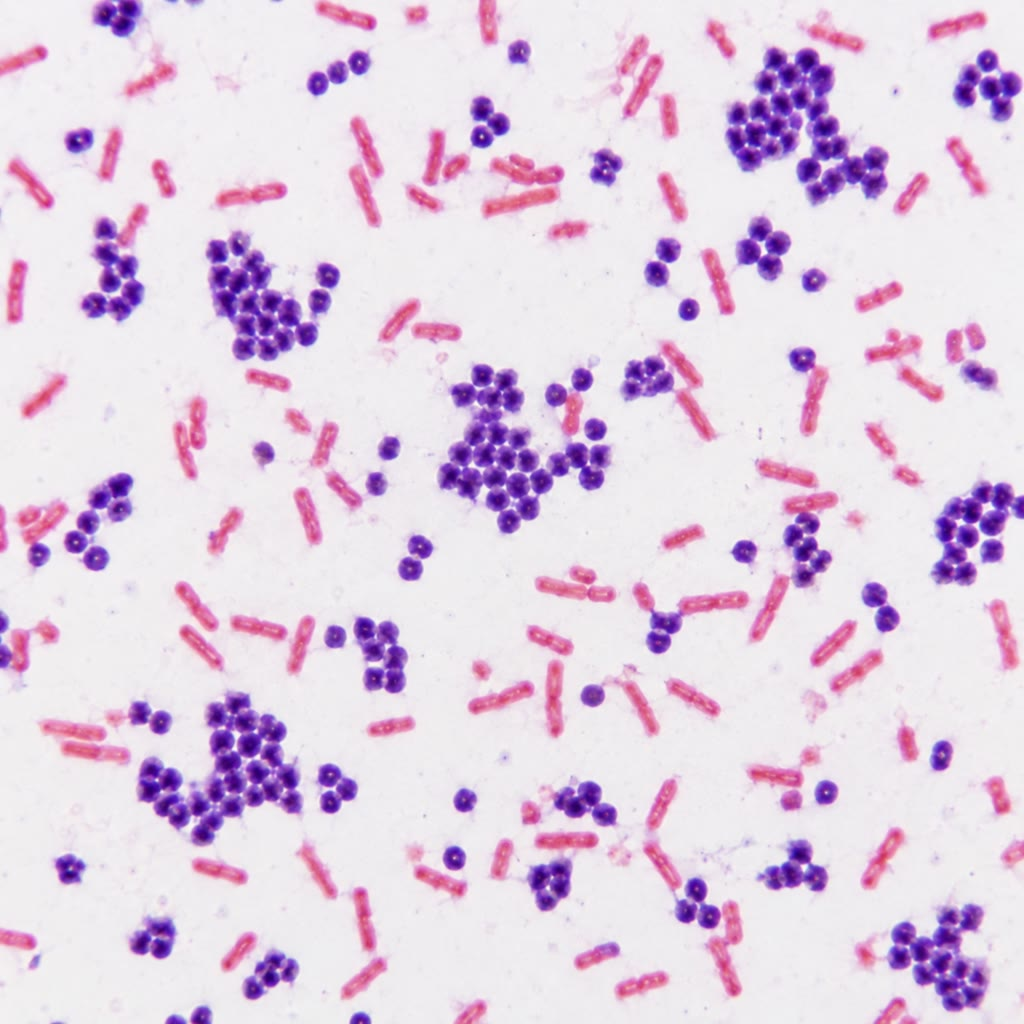
\includegraphics[width=0.36\linewidth]{images/book5/ai/b5-12-gram-stain.jpg}\hspace{0.04\linewidth}
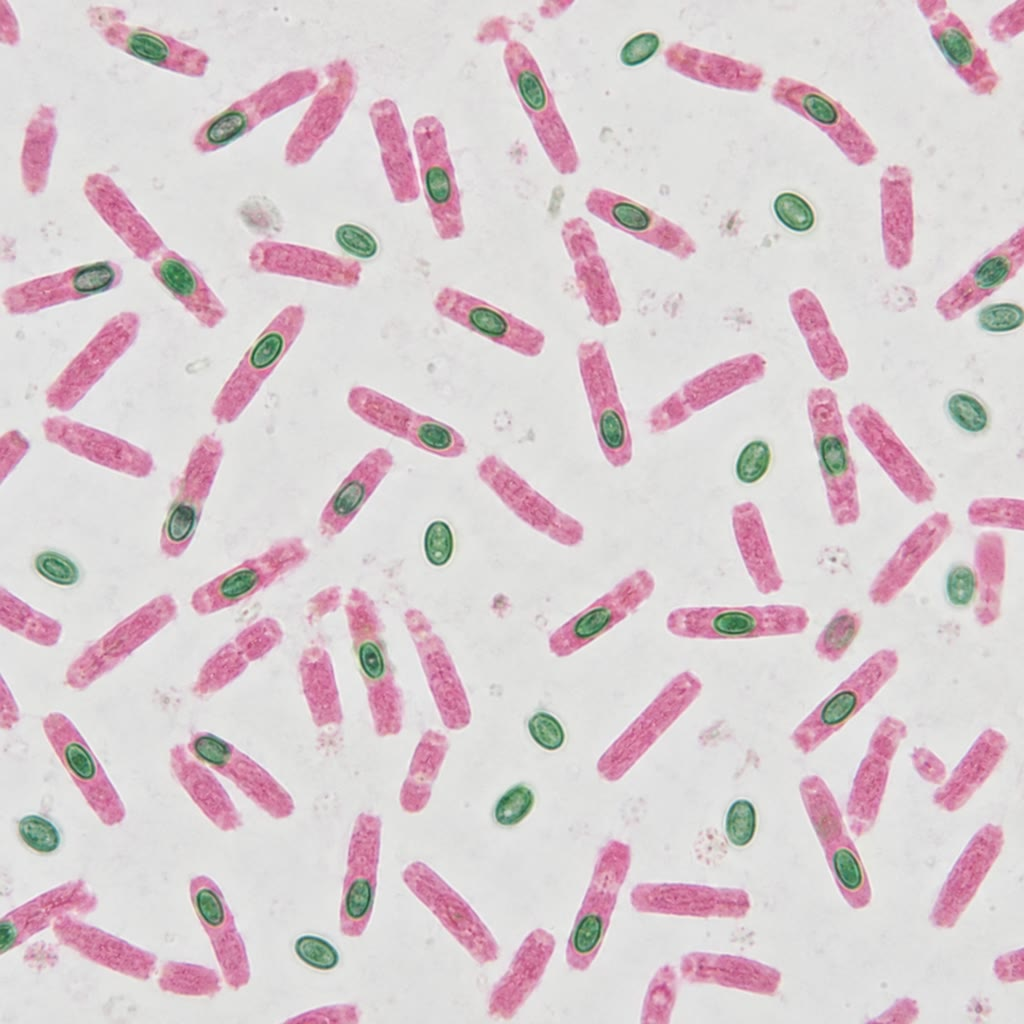
\includegraphics[width=0.36\linewidth]{images/book5/ai/b5-12-endospores.jpg}

{\small يسارًا: \omterm{met:b3:bacteriology:gram}{صبغة غرام} --- مكورات إيجابية الغرام بنفسجية في عناقيد،
وعصيات سلبية الغرام وردية. يمينًا: خلايا \emph{Bacillus} مصبوغة لإظهار
الأبواغ الداخلية، وهي البيضاويات الخضر الساطعة داخل خلايا وردية وأبواغ حرة
بجانبها.}
\end{omfigure}

\begin{omfigure}
\begin{tikzpicture}[every node/.style={font=\scriptsize}, >=stealth]
  % Gram-positive
  \begin{scope}
    \fill[omDef!15] (0,0) rectangle (4.5,0.4); \draw[thick, omDef] (0,0) -- (4.5,0); \draw[thick, omDef] (0,0.4) -- (4.5,0.4);
    \fill[omProp!40] (0,0.5) rectangle (4.5,2.0); \foreach \y in {0.7,0.95,1.2,1.45,1.7} \draw[omProp!80!black, thin] (0,\y) -- (4.5,\y);
    \foreach \x in {0.6,1.6,2.6,3.6} \draw[omMeth!70!black, thick] (\x,0.5) -- (\x,2.3);
    \node[below] at (2.25,-0.1) {الغشاء الهيولي};
    \node[right, align=left] at (4.6,1.25) {ببتيدوغليكان ثخين\\(\qtyrange{20}{80}{nm})}; \node[right, omMeth!70!black] at (4.6,2.2) {حموض التيكويك};
    \node[above, font=\small\bfseries] at (2.25,2.5) {إيجابية الغرام};
  \end{scope}
  % Gram-negative
  \begin{scope}[xshift=8.6cm]
    \fill[omDef!15] (0,0) rectangle (4.5,0.4); \draw[thick, omDef] (0,0) -- (4.5,0); \draw[thick, omDef] (0,0.4) -- (4.5,0.4);
    \fill[omProp!40] (0,0.75) rectangle (4.5,1.05); \draw[omProp!80!black, thin] (0,0.9) -- (4.5,0.9);
    \fill[omDef!15] (0,1.5) rectangle (4.5,1.9); \draw[thick, omDef] (0,1.5) -- (4.5,1.5); \draw[thick, omDef] (0,1.9) -- (4.5,1.9);
    \foreach \x in {0.4,0.9,1.4,1.9,2.4,2.9,3.4,3.9} \draw[omThm, thick] (\x,1.9) -- (\x,2.35);
    \draw[thick, fill=white] (2.0,1.45) rectangle (2.5,1.95); \node[below, font=\tiny] at (2.25,1.45) {بورين};
    \node[below] at (2.25,-0.1) {الغشاء الهيولي};
    \node[right] at (4.6,0.9) {ببتيدوغليكان رقيق}; \node[right] at (4.6,1.7) {غشاء خارجي}; \node[right, omThm] at (4.6,2.25) {LPS (ذيفان داخلي)};
    \node[right, font=\tiny] at (4.6,1.27) {المحيط حول البلازما};
    \node[above, font=\small\bfseries] at (2.25,2.5) {سلبية الغرام};
  \end{scope}
\end{tikzpicture}

{\small الغلافان. إيجابيات الغرام تلف الغشاء بطبقات
كثيرة من \omterm{def:b3:bacteriology:envelope}{الببتيدوغليكان}؛ وسلبيات الغرام لها طبقة رقيقة \omterm{def:b3:bacteriology:envelope}{وغشاء
خارجي} من \omterm{def:b3:bacteriology:envelope}{عديد السكريد الشحمي} تخترقه البورينات، وهو يبقي كثيرًا من
المضادات الحيوية في الخارج ويصنع الذيفان الداخلي الذي يسبب الصدمة الإنتانية.}
\end{omfigure}

\section{النمو}

\begin{theorem}[النمو الأسّي وقانون مونو والمزرعة الكيميائية المستقرة]\label{thm:b3:bacteriology:monod}
\index{نمو أسّي!في البكتيريا}\index{معادلة مونو}\index{مزرعة كيميائية مستقرة}\index{معدل التمديد}
جمهرة من $N$ خلية تنقسم بزمن جيل $T$ تنمو بحسب
$N(t) = N_{0}\,2^{t/T} = N_{0}e^{\mu t}$ بمعدل نمو نوعي $\mu =
\ln 2/T$. ويتوقف المعدل على المغذي المحدِّد $S$ بحسب
\emph{قانون مونو}
\[
\mu(S) = \mu_{\max}\,\frac{S}{K_{S} + S},
\]
وهو يتشبع عند $\mu_{\max}$ ويبلغ نصف أقصاه عند $S = K_{S}$. وفي
\emph{\omterm{thm:b3:bacteriology:monod}{المزرعة الكيميائية المستقرة}} --- وهي وعاء حجمه $V$ يدخله وسط طازج
تركيز مغذيه $S_{0}$ بمعدل $F$، وتخرج منه
المزرعة بالمعدل نفسه، \omterm{thm:b3:bacteriology:monod}{ومعدل التمديد} $D = F/V$ ---
تكون الحالة المستقرة
\[
\mu(S^{*}) = D,\qquad S^{*} = \frac{K_{S}D}{\mu_{\max} - D},\qquad
X^{*} = Y\,(S_{0} - S^{*}),
\]
حيث $X$ كثافة الخلايا و$Y$ الغلة (أي الخلايا المصنوعة لكل وحدة من
المغذي). فالمجرّب يضبط معدل النمو بإدارة مضخة؛
والمزرعة تستجيب بضبط المغذي الذي تتركه خلفها. وإذا تجاوزت $D$
القيمة $\mu(S_{0})$ عجزت الخلايا عن مواكبتها وغُسلت خارجًا.
\end{theorem}
\begin{proof}
الخلايا: $\mathrm{d}X/\mathrm{d}t = \mu(S)X - DX$، أي النمو ناقص الخروج؛
وعند الحالة المستقرة مع $X^{*} > 0$، يكون $\mu(S^{*}) = D$، وقلبُ
قانون مونو يعطي $S^{*}$. والمغذي: $\mathrm{d}S/\mathrm{d}t = D(S_{0} -
S) - \mu(S)X/Y$، أي الدخول ناقص الخروج ناقص الاستهلاك؛ وعند الحالة
المستقرة، مع $\mu = D$، يكون $D(S_{0} - S^{*}) = DX^{*}/Y$، ومنه $X^{*}$.
ولا توجد الحالة المستقرة إلا إذا كانت $S^{*} < S_{0}$، أي $D <
\mu(S_{0})$؛ وبعد ذلك تكون الحالة المستقرة الوحيدة $X = 0$، أي الغسل.
والاستقرار: فإذا ارتفعت $X$ فوق $X^{*}$ استهلكت أكثر، فهبطت $S$ دون
$S^{*}$، وهبطت $\mu$ دون $D$ وتناقصت $X$ --- أي تغذية راجعة سالبة
عبر المغذي.
\end{proof}

\begin{example}[مزرعة بالأرقام]\label{ex:b3:bacteriology:numbers}
\emph{E.~coli} في وسط غني عند \qty{37}{\celsius}: $T = \qty{20}{min}$،
و$\mu = \qty{2.1}{h^{-1}}$. فمن خلية واحدة، $2^{36}$ بعد اثنتي عشرة ساعة
--- أي $7\times 10^{10}$ خلية، ونحو \qty{70}{mg}، وهو حيث يتوقف دورق
سعته \qty{100}{mL} لنفاد الأكسجين والسكر؛ و``كتلة
الأرض في يومين'' هي $2^{144}\approx 10^{43}$ خلية، و
الحساب لا يبيّن إلا أن النمو الأسّي لا يدوم أبدًا. وفي
مزرعة كيميائية على الغلوكوز عند $\mu_{\max} = \qty{1.0}{h^{-1}}$، و$K_{S} =
\qty{0.01}{g/L}$، و$S_{0} = \qty{1}{g/L}$، و$Y = \qty{0.5}{g}$ من الخلايا
لكل غرام غلوكوز، يترك معدل تمديد قدره \qty{0.5}{h^{-1}} قيمة $S^{*}
= 0.01\times 0.5/0.5 = \qty{0.01}{g/L}$ من الغلوكوز ويحفظ $X^{*} =
\qty{0.495}{g/L}$ من الخلايا، تنقسم كل \qty{83}{min}، بلا حد.
\omterm{thm:b3:bacteriology:monod}{والمزرعة الكيميائية المستقرة} هي كيف تُدرس فيزيولوجيا معدل نمو ثابت،
وكيف تُجرى آلاف الأجيال من التطور في قنينة.
\end{example}

\begin{omfigure}
\begin{tikzpicture}
\begin{axis}[
  width=6.6cm, height=5.4cm,
  axis x line=bottom, axis y line=left,
  xmin=0, xmax=14, ymin=1e6, ymax=1e10, ymode=log,
  xlabel={الساعات}, ylabel={خلايا في المليلتر},
  xlabel style={font=\small, at={(axis description cs:0.5,-0.12)}, anchor=north}, ylabel style={font=\small},
  tick label style={font=\scriptsize}, xtick={0,4,8,12},
  clip=false,
]
\addplot[very thick, omDef, domain=0:1.5, samples=2] {1e6};
\addplot[very thick, omDef, domain=1.5:7.5, samples=40] {1e6*2^((x-1.5)/0.5)};
\addplot[very thick, omDef, domain=7.5:12, samples=2] {4.1e9};
\addplot[very thick, omDef, domain=12:14, samples=10] {4.1e9*exp(-0.15*(x-12))};
\node[font=\scriptsize, anchor=south] at (axis cs:0.8,1.2e6) {تلكؤ};
\node[font=\scriptsize, anchor=west] at (axis cs:2.5,3e8) {أسّي: $T = \qty{30}{min}$};
\node[font=\scriptsize, anchor=north] at (axis cs:10,3.5e9) {ثابت};
\node[font=\scriptsize, anchor=north] at (axis cs:12.8,2.2e9) {موت};
\end{axis}
\begin{axis}[
  at={(7.8cm,0)}, anchor=south west,
  width=6.6cm, height=5.4cm,
  axis x line=bottom, axis y line=left,
  xmin=0, xmax=0.1, ymin=0, ymax=1.1,
  xlabel={الغلوكوز $S$ (g/L)}, ylabel={$\mu$ (h$^{-1}$)},
  xlabel style={font=\small, at={(axis description cs:0.5,-0.12)}, anchor=north}, ylabel style={font=\small},
  tick label style={font=\scriptsize}, xtick={0,0.01,0.05,0.1}, xticklabels={0,$K_S$,0.05,0.1}, ytick={0,0.5,1},
  clip=false,
]
\addplot[very thick, omThm, domain=0:0.1, samples=60] {x/(0.01+x)};
\addplot[dashed, gray, domain=0:0.1, samples=2] {1};
\addplot[dashed, gray] coordinates {(0.01,0) (0.01,0.5)}; \addplot[dashed, gray] coordinates {(0,0.5) (0.01,0.5)};
\node[font=\scriptsize, omThm, anchor=north west] at (axis cs:0.045,0.6) {مونو: $\mu = \mu_{\max}S/(K_{S}+S)$};
\node[font=\scriptsize, gray, anchor=south east] at (axis cs:0.1,1.01) {$\mu_{\max}$};
\end{axis}
\end{tikzpicture}

{\small يسارًا: مزرعة دفعة --- تلكؤ ريثما تُحرَّض الإنزيمات، ثم
نمو أسّي، وطور ثابت حين ينفد المغذي، ثم
موت بطيء. يمينًا: قانون مونو، معدل النمو في مقابل المغذي
المحدِّد، و$K_{S}$ هو التركيز عند نصف النمو الأقصى.}
\end{omfigure}

\begin{definition}[الأطوار والحالات]\label{def:b3:bacteriology:phases}
\index{طور التلكؤ}\index{الطور الثابت}\index{التبوغ}\index{عامل سيغما}
في دورق طازج (وهي \emph{مزرعة الدفعة}) تتوقف الخلايا أولًا --- وهو
\emph{طور التلكؤ}، ريثما تحرّض الإنزيمات التي يحتاجها الوسط الجديد
--- ثم تنمو أسّيًا، ثم تتوقف حين ينفد مغذٍّ أو
تتراكم فضلة: وهو \emph{الطور الثابت}، تنكمش فيه الخلايا، و
تثخّن غلافها، وتكثّف نُوَيدها حول بروتينات
واقية، وتفتح مورّثات الكرب عبر عامل سيغما
البديل RpoS، وتستطيع أن تبقى شهورًا؛ ويتبعه طور موت
تنحل فيه معظم الخلايا ويعيش قليل منها على البقايا. وبعض الأنواع
يجيب عن الجوع ببرنامج تطوري: فالنوع \emph{Bacillus
subtilis} ينقسم انقسامًا غير متناظر وتبتلع الخلية الأكبر
الأصغر وتبني البوغ حولها، في تسلسل من ثماني ساعات
يتحكم فيه شلال من \emph{عوامل سيغما} --- وهي الوحدات التي
توجّه بوليميراز RNA إلى طقم من المروّجات --- بالتناوب بين
المقصورتين، وهو أول مثال بكتيري على التمايز
وعلى الإشارة بين خلية وأخرى عبر جدار.
\end{definition}

\section{استشعار بعضها بعضًا}

\begin{definition}[استشعار النصاب]\label{def:b3:bacteriology:quorum}
\index{استشعار النصاب}\index{محرّض ذاتي}\index{منظومة ثنائية المكوّن}
تكشف البكتيريا كثافتها هي عبر \emph{استشعار النصاب}: فكل خلية
تفرز جزيء إشارة صغيرًا، وهو \emph{محرّض ذاتي} --- لاكتونات
الهوموسيرين المؤسترة في سلبيات الغرام، وببتيدات قصيرة في إيجابيات الغرام
--- بمعدل ثابت؛ ويرتفع التركيز في الوسط مع
عدد الخلايا، فإذا تجاوز عتبةً ارتبط بمستقبل
يفتح طقمًا من المورّثات، منها سينثاز
المحرّض الذاتي نفسه (ومن هنا الاسم). والمورّثات المتحكَّم فيها هكذا هي
التي لا تفيد إلا في جماعة: كالضوء في \emph{Vibrio fischeri}،
وعوامل الفوعة في \emph{Staphylococcus aureus} و
\emph{Pseudomonas aeruginosa}، وحشوة الغشاء الحيوي، والكفاءة لالتقاط
DNA، وقتل الجيران. ومعظم استشعار البكتيريا يجري
عبر \emph{منظومات ثنائية المكوّن}: كيناز هستيديني غشائي
يكشف منبّهًا ويفسفر منظّم استجابة هيوليًا،
يرتبط بجزيء DNA --- ولدى الخلية عشرات منها، للفوسفات، والأسمولية، و
الأكسجين، ومحرّضات الأنواع الأخرى.
\end{definition}

\begin{proof}[شواهد]
نمّى نيلسون وبلات وهاستنغز (1970) البكتيريا البحرية المضيئة
\emph{Vibrio fischeri} من لقاح ممدَّد فوجدوا أن الخلايا
لا تصنع ضوءًا حتى تبلغ كثافة قدرها نحو $10^{7}$ في
المليلتر، ثم تضيء كلها معًا؛ وأن وسطًا نمت فيه مزرعة كثيفة،
ثم عُقّم وأُضيف إلى مزرعة ممددة، فتح الضوء
فورًا. فالخلايا كانت تعدّ مادة مفرَزة، لا زمنًا ولا
مغذيًا. وحُدّدت المادة لاكتون أسيل هوموسيرين
(إبرهارد، 1981)، واستُنسخت المورّثات --- \emph{luxI} للسينثاز، و
\emph{luxR} للمستقبل، وأوبرون اللوسيفيراز الذي تتحكم فيه ---
في \emph{E.~coli}، فصارت تتوهج حين تزدحم. وفي
الحبار الذي يؤوي البكتيريا عند $10^{10}$ في المليلتر، يضيء
عضو الضوء؛ وفي البحر، حيث تكون البكتيريا ممددة، تكون
مظلمة وتوفّر الكلفة.
\end{proof}

\begin{proposition}[عتبة كثافة]\label{prop:b3:bacteriology:threshold}
\index{استشعار النصاب!العتبة}
لتفرز كل خلية من $N$ خلية في حجم $V$ محرّضًا ذاتيًا بمعدل $p$
جزيء في الثانية، وليُفقد الجزيء (بالتحلل أو
التمديد) بمعدل من الرتبة الأولى $k$. عندئذٍ يقترب التركيز من
$A^{*} = pN/(kV)$، متناسبًا مع كثافة الخلايا $N/V$، بثابت
زمن $1/k$؛ ويُفتح المستقبل حين تبلغ $A^{*}$
عتبته $A_{\text{thr}}$، أي عند الكثافة
\[
\left(\frac{N}{V}\right)_{\text{thr}} = \frac{k\,A_{\text{thr}}}{p}.
\]
وفي حيز مغلق --- كعضو ضوء حبار، أو خُراج، أو مخاط
رئة --- تكون $k$ صغيرة لأن الإشارة لا تُحمل بعيدًا، فتُبلغ
الكثافة العتبية بخلايا أقل؛ وفي الماء المفتوح لا تُبلغ
أبدًا. فالخلية تقيس إذن لا عددها بل عددها
لكل وحدة من الحجم الذي تشارك فيه، وهو ما يهم في
أي فعل تعاوني، والتغذية الراجعة الموجبة \omterm{def:b3:bacteriology:quorum}{للمحرّض الذاتي} على
سينثازه هو تجعل المفتاح حادًا: فمتى تجاوزت بضع خلايا
العتبة، دفع ناتجها الزائد البقيةَ فوقها.
\end{proposition}
\begin{proof}
$\mathrm{d}A/\mathrm{d}t = pN/V - kA$ لها الحالة المستقرة $A^{*} =
pN/(kV)$ وتسترخي إليها مثل $e^{-kt}$. ووضعُ $A^{*} = A_{\text{thr}}$
والحل من أجل $N/V$ يعطي الكثافة العتبية.
\end{proof}

\begin{omfigure}
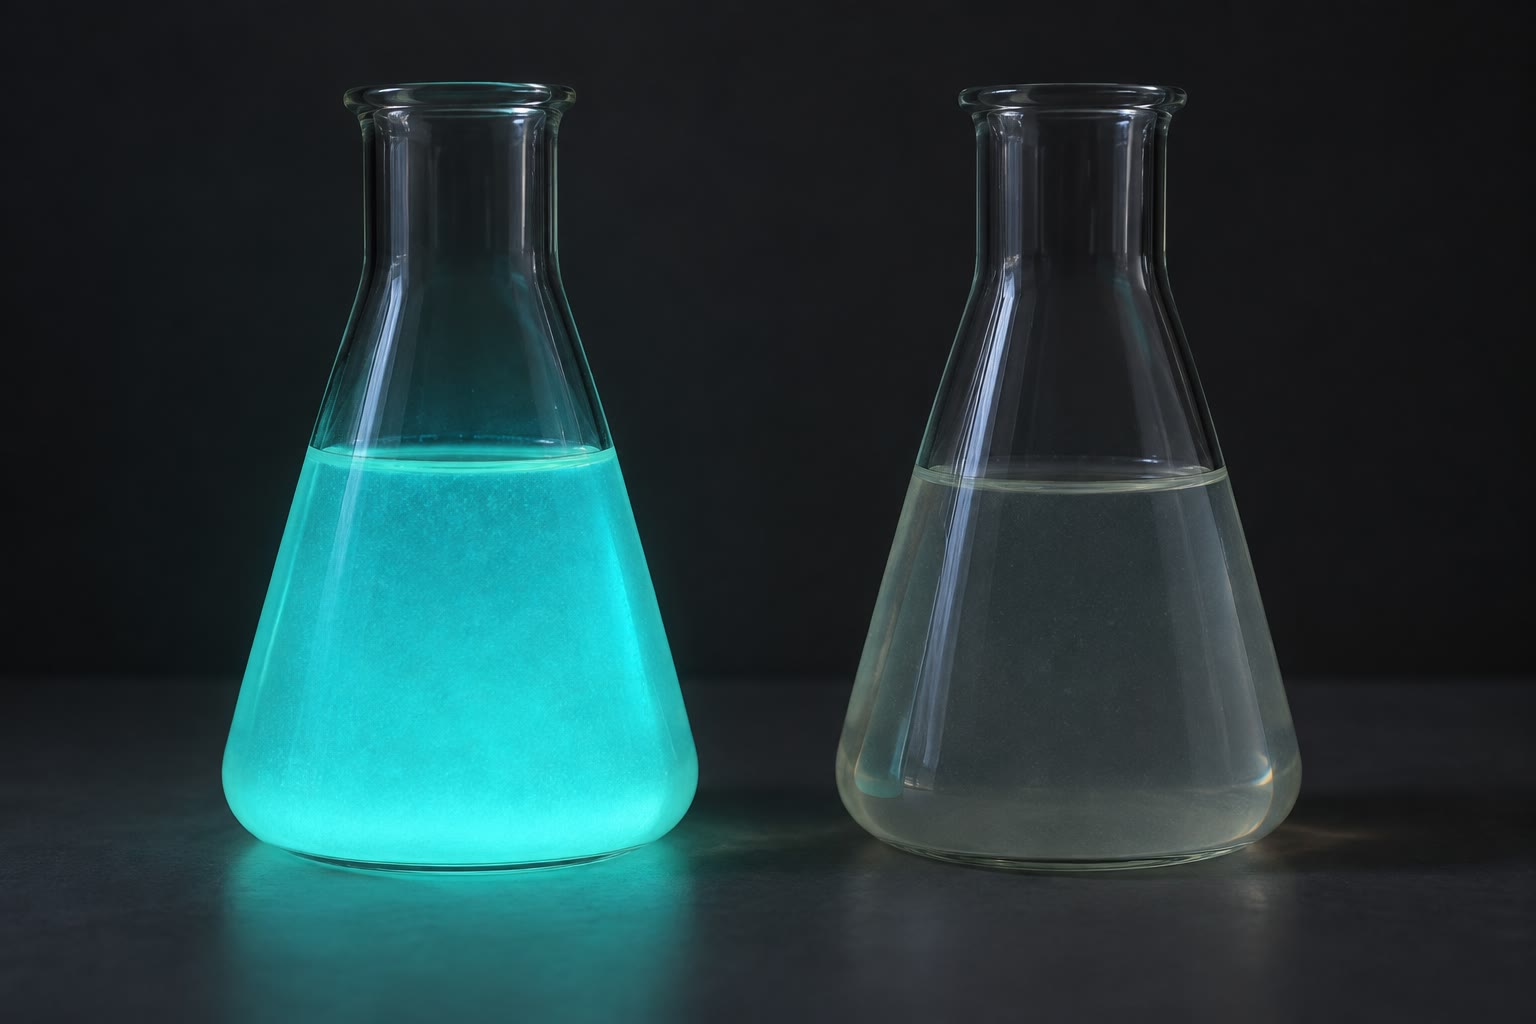
\includegraphics[width=0.46\linewidth]{images/book5/ai/b5-12-quorum-glow.jpg}\hspace{0.04\linewidth}
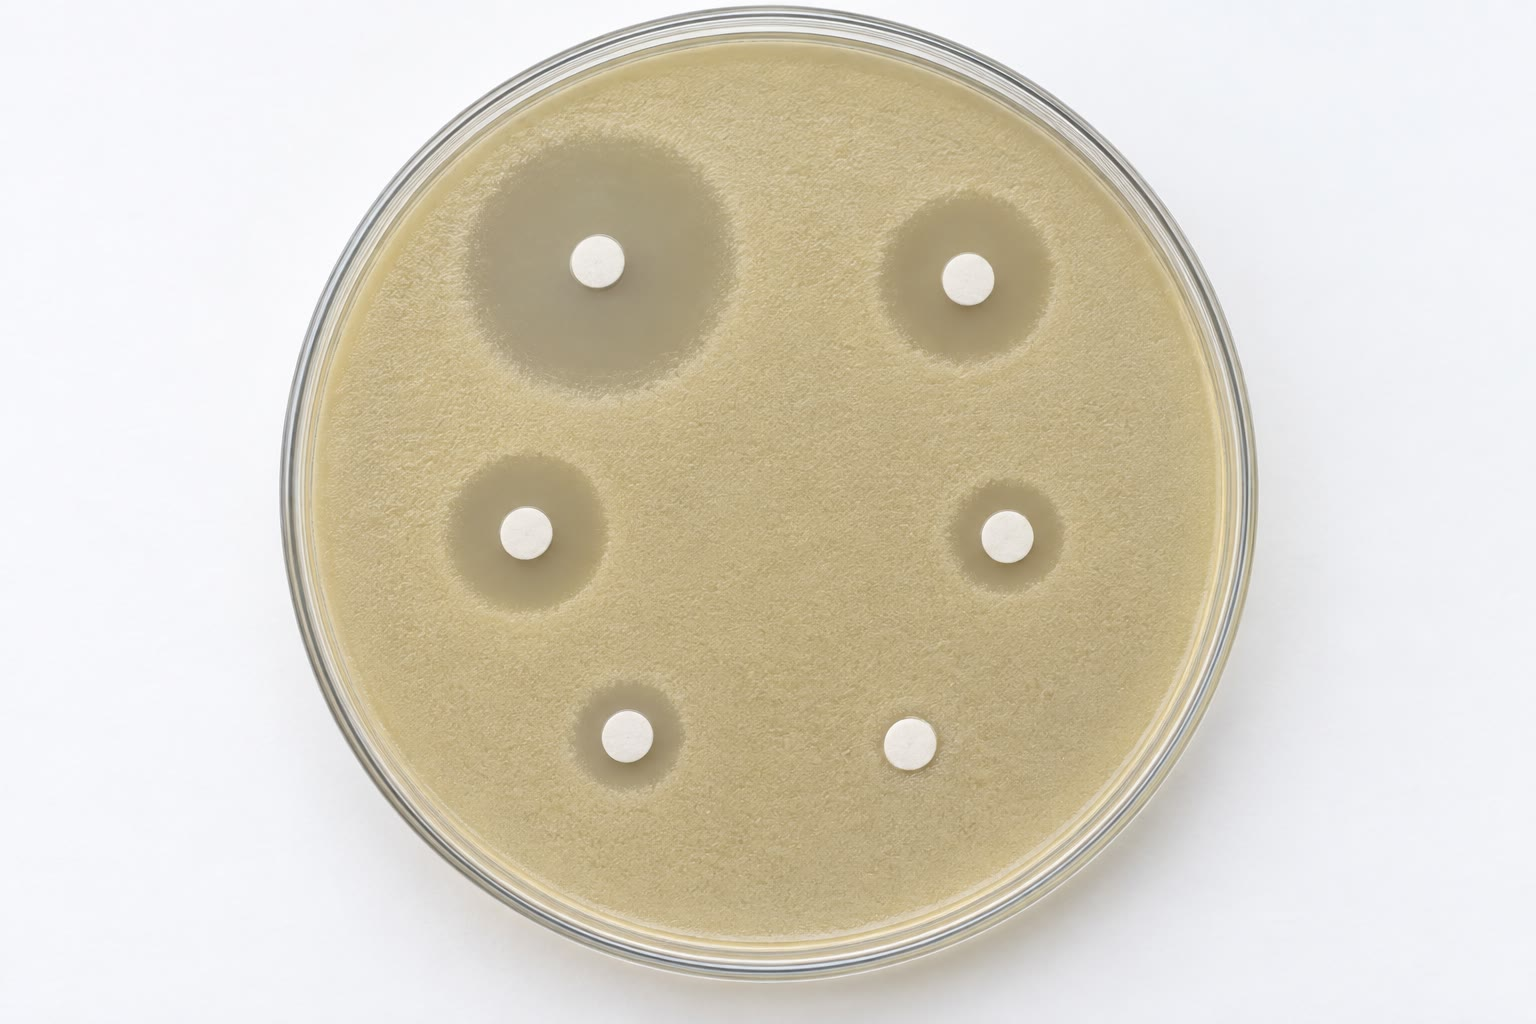
\includegraphics[width=0.46\linewidth]{images/book5/ai/b5-12-antibiotic-disks.jpg}

{\small يسارًا: مزرعة كثيفة من \emph{Vibrio fischeri} متوهجة، بجانب
مزرعة ممددة مظلمة --- وهي الخلايا نفسها، فوق نصابها وتحته.
يمينًا: اختبار \omterm{met:b3:bacteriology:mic}{انتشار الأقراص}؛ فقطر كل منطقة صافية
يقيس حساسية البكتيريا \omterm{def:b3:bacteriology:antibiotics}{للمضاد الحيوي} على ذلك القرص،
والقرص الذي لا منطقة له يعلّم مقاومة.}
\end{omfigure}

\section{حركة المورّثات}

\begin{definition}[النقل الأفقي للمورّثات]\label{def:b3:bacteriology:hgt}
\index{تحول}\index{نقل بالعاثيات}\index{اقتران}\index{بلازميد!المقاومة}\index{عنصر وراثي متنقل}\index{الجينوم الشامل}
تتكاثر البكتيريا نسيليًا لكنها تتبادل المورّثات بثلاثة طرق.
\emph{التحول}: التقاط DNA عارٍ من البيئة بخلية
كفؤة --- وهو الطريق الذي اكتسبت به مكورات غريفيث الرئوية
محفظتها وبيّن به آفري أن مبدأ التحول DNA
(1944). و\emph{النقل بالعاثيات}: عاثية تحزم قطعة من DNA المضيف
وتحقنها في المضيف التالي (\cref{ch:b3:virology}).
و\emph{الاقتران}: نقل \omterm{def:b3:genetic-engineering:tools}{بلازميد} عبر هلب وجسر
تزاوج من مانح يحمله إلى متلقٍّ، وقد بيّنه
ليدربرغ وتاتوم (1946) بسلالات معوزة من \emph{E.~coli}
لم تعط مؤتلفات مكتفية إلا حين خُلطت. والبلازميدات
الاقترانية تحمل مورّثات نقلها هي؛ وكثير منها يحمل أيضًا مورّثات
مقاومة، متجمعة غالبًا في \emph{الإنتغرونات} ومحفوفة بعناصر قافزة،
حتى إن تزاوجًا واحدًا يستطيع أن ينقل مقاومة خمسة مضادات حيوية
دفعةً واحدة، عبر الأنواع. والنتيجة أن للنوع البكتيري
جينومًا لبّيًا تشترك فيه السلالات كلها وجينومًا ملحقًا
متغيرًا --- وهو \emph{الجينوم الشامل}: فقد تختلف سلالتان من \emph{E.~coli} في
خمس مورّثاتهما، وتختلف السلالات الممرضة عن غير الضارة
أساسًا بجزر فوعة مكتسبة. ومورّثات
فصل الطفرات في كتاب السنة~الثانية تنشأ بالطفرة؛ أما مورّثات هذا
الفصل فتصل في معظمها وصولًا.
\end{definition}

\begin{omfigure}
\begin{tikzpicture}[every node/.style={font=\scriptsize}, >=stealth]
  % transformation
  \begin{scope}
    \draw[thick, fill=omDef!15] (0,0) ellipse (1.0 and 0.55);
    \draw[omThm, very thick] (-1.9,0.6) .. controls (-1.5,0.8) .. (-1.2,0.5); \draw[->, omThm, thick] (-1.2,0.5) -- (-0.7,0.25);
    \node[below, align=center] at (0,-0.7) {التحول:\\DNA عارٍ تلتقطه\\خلية كفؤة};
  \end{scope}
  % transduction
  \begin{scope}[xshift=4.6cm]
    \draw[thick, fill=omDef!15] (0,0) ellipse (1.0 and 0.55);
    \draw[thick, fill=omProp!40] (-1.3,1.0) -- (-1.0,1.3) -- (-0.7,1.0) -- (-1.0,0.7) -- cycle; \draw[thick] (-1.0,0.7) -- (-0.9,0.35);
    \draw[omThm, very thick] (-1.1,1.15) -- (-0.9,0.85);
    \node[below, align=center] at (0,-0.7) {النقل بالعاثيات:\\عاثية تحمل قطعة\\من DNA مضيفها الأخير};
  \end{scope}
  % conjugation
  \begin{scope}[xshift=9.6cm]
    \draw[thick, fill=omDef!15] (-1.3,0) ellipse (0.9 and 0.5); \draw[thick, fill=omDef!15] (1.3,0) ellipse (0.9 and 0.5);
    \draw[very thick, omMeth!70!black] (-0.4,0) -- (0.4,0);
    \draw[omThm, very thick] (-1.5,0) circle (0.25); \draw[->, omThm, thick] (-1.25,0) -- (1.0,0);
    \node[below, align=center] at (0,-0.7) {الاقتران:\\بلازميد يعبر\\جسر تزاوج};
  \end{scope}
\end{tikzpicture}

{\small طرق النقل الأفقي الثلاثة. فمورّثات المقاومة
والفوعة والاستقلاب تنتقل بين الخلايا --- وبين الأنواع ---
أسرع مما تستطيع الطفرة أن تصنعها.}
\end{omfigure}

\begin{proof}[شواهد]
أثبت روبرت كوخ (1876--1884) أن بكتيريا بعينها تسبب
مرضًا بعينه: فعزل \emph{Bacillus anthracis} من حيوانات
مريضة، ونمّاها مزرعةً نقية على وسط صلب (وطبق الأغار و
المستعمرة المفردة من ابتكارات مختبره)، وبيّن أن
المزرعة تعيد إنتاج الجمرة الخبيثة في حيوانات سليمة ويمكن إعادة عزلها
منها --- وهي المسلّمات التي ما تزال تعرّف الممرض --- ثم مضى
إلى عصية السل وضمة الكوليرا. ولاحظ ألكسندر فلمنغ
(1928) أن عفنًا لوّث طبقًا من العنقوديات كان قد
صفّى منطقة حوله؛ ونُقّيت المادة، وهي البنسلين،
وبيّن فلوري وتشين (1940--1941) أنها تشفي الأخماج، و
في غضون عقد شاعت في المستشفيات عنقوديات مقاومة تحمل
إنزيمًا يهدم البنسلين --- وهو تحذير أطلقه فلمنغ نفسه في
محاضرة نوبل.
\end{proof}

\begin{omfigure}
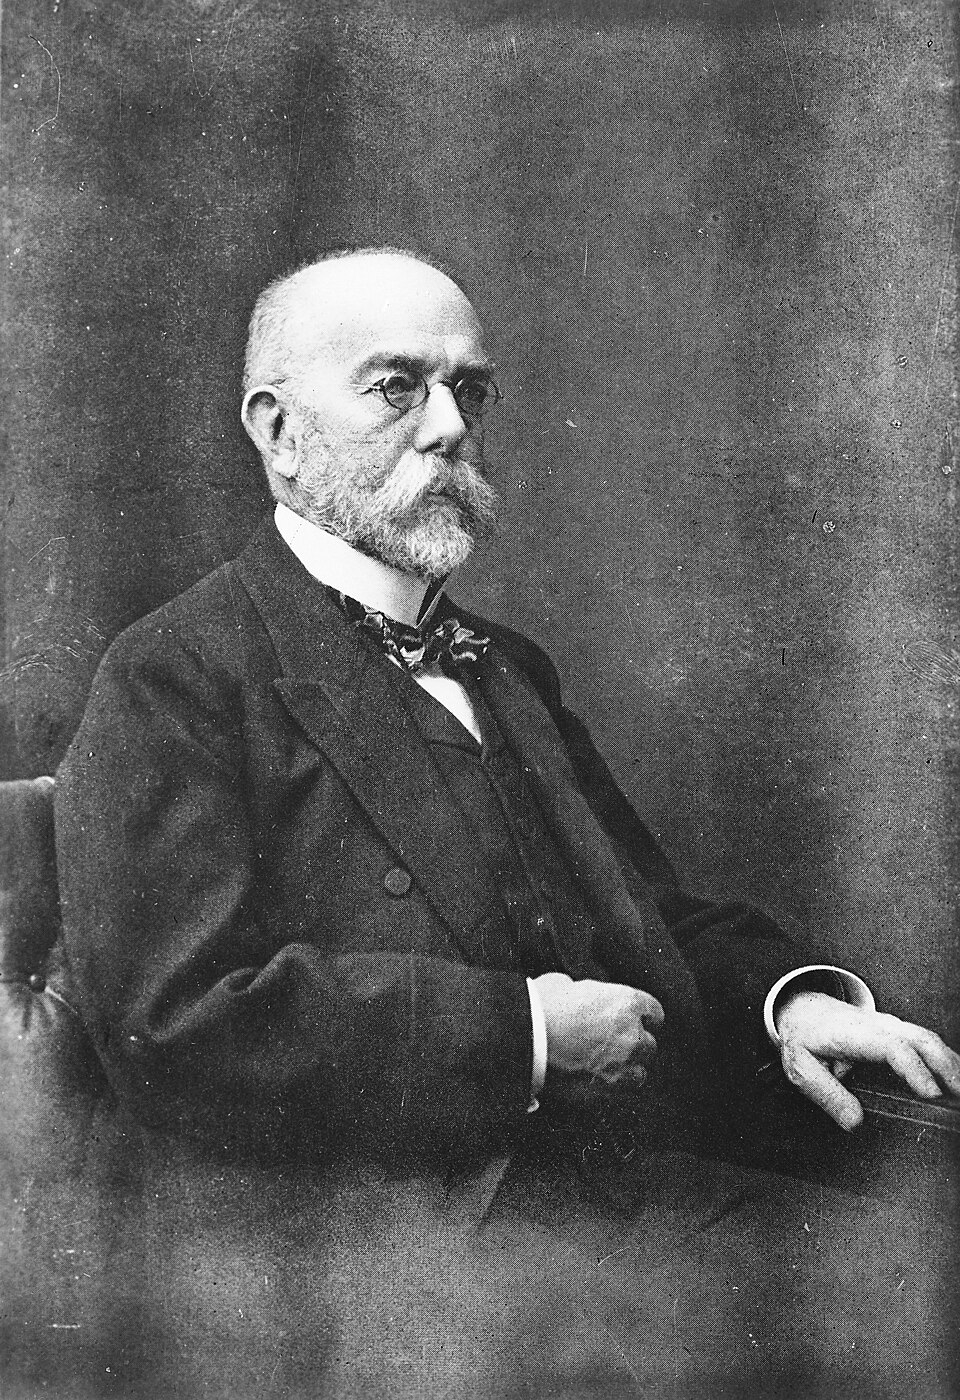
\includegraphics[width=0.30\linewidth]{images/book5/koch.jpg}\hspace{0.04\linewidth}
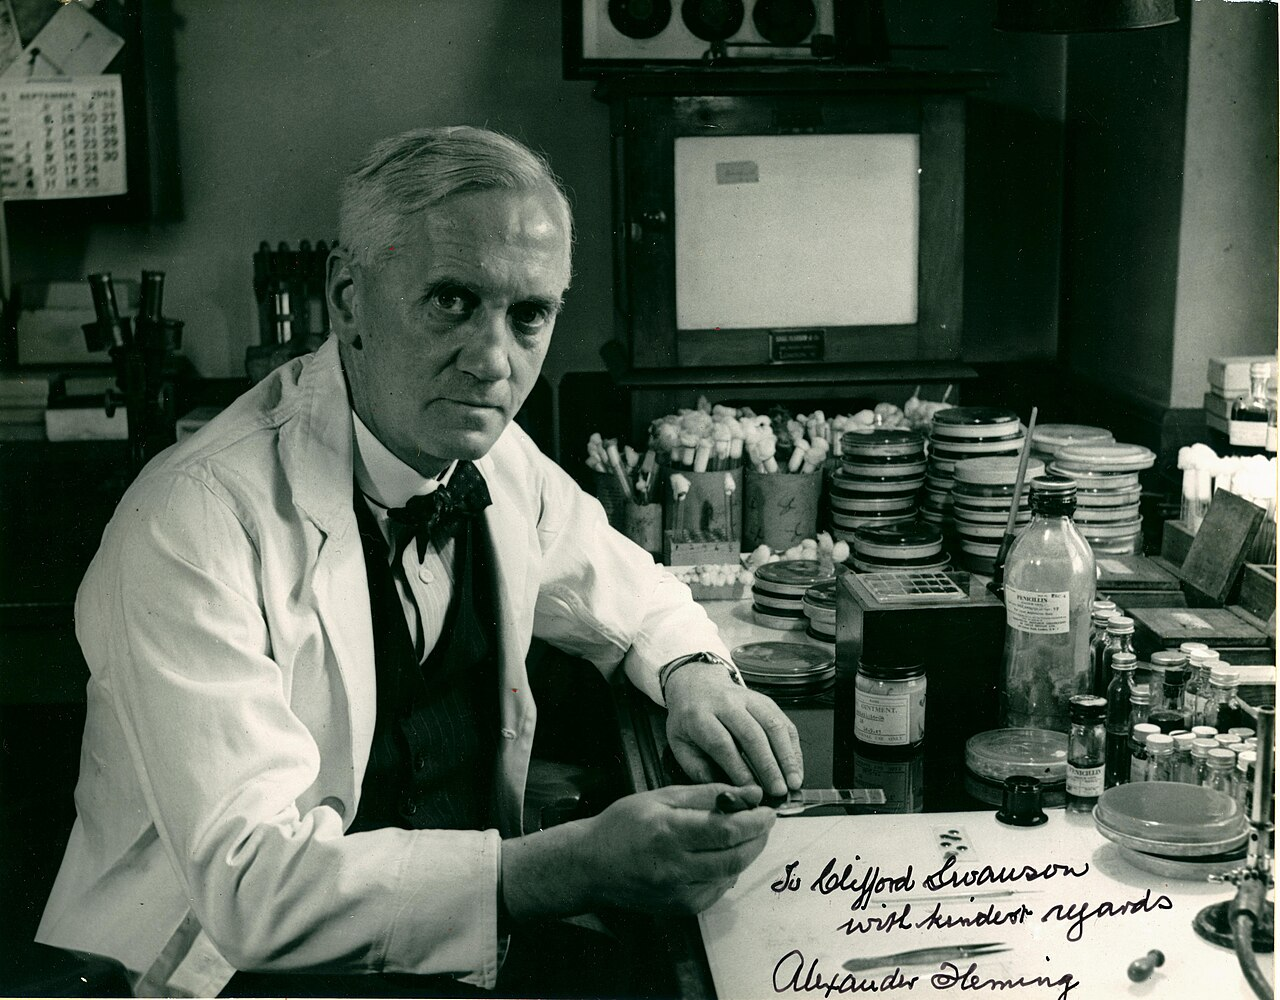
\includegraphics[width=0.56\linewidth]{images/book5/fleming.jpg}

{\small روبرت كوخ، الذي برهن على أن بكتيريا بعينها تسبب
أمراضًا بعينها وابتكر طرائق تنميتها (Wellcome
Collection، رخصة CC~BY~4.0). يمينًا: ألكسندر فلمنغ في مختبره
مع أطباق العفن الذي صار ناتجه البنسلين (أرشيف بحرية الولايات
المتحدة، ملكية عامة).}
\end{omfigure}

\section{المضادات الحيوية والمقاومة}

\begin{definition}[المضادات الحيوية]\label{def:b3:bacteriology:antibiotics}
\index{مضاد حيوي}\index{بيتا-لاكتام}\index{سمية انتقائية}\index{أدنى تركيز مثبط}
\emph{المضاد الحيوي} جزيء يقتل البكتيريا أو يوقف
نموها عند تراكيز لا تضر المضيف، بعمله على هدف
يخلو منه المضيف أو يملكه بصورة مختلفة --- وهي \emph{السمية
الانتقائية}. والأهداف قليلة. فجدار الخلية: \emph{$\beta$-اللاكتامات}
(البنسلينات، والسيفالوسبورينات، والكاربابينيمات) تحاكي طرف
D-Ala-D-Ala في ببتيد \omterm{def:b3:bacteriology:envelope}{الببتيدوغليكان} وتؤستل الإنزيمات التي
تشبّكه، فيكون الجدار النامي ضعيفًا وتنفجر الخلية
تحت امتلائها؛ والفانكوميسين يربط D-Ala-D-Ala نفسه. و
الريبوزوم، وصورته البكتيرية تختلف عن صورة حقيقيات النوى: فالأمينوغليكوزيدات
(الوحدة الصغيرة، فتسبب سوء القراءة)، والتتراسيكلينات (بحجب دخول
tRNA)، والماكروليدات والكلورامفينيكول (نفق خروج الوحدة الكبيرة
وناقلة الببتيديل). وجيراز DNA والتوبوإيزوميراز~IV:
الكينولونات. وبوليميراز RNA: الريفامبيسين. واصطناع الفولات، وهو ما
لا تفعله الحيوانات: السلفوناميدات والتريميثوبريم. والغشاء:
البوليميكسينات، وهي الملاذ الأخير. و\emph{أدنى تركيز مثبط}
(MIC) هو أخفض تركيز من دواء يمنع نموًا مرئيًا
لسلالة؛ وتُسمى السلالة مقاومة حين يتجاوز MIC عندها
التركيزَ الذي يبلغه الدواء في المريض.
\end{definition}

\begin{method}[قياس الحساسية]\label{met:b3:bacteriology:mic}
\index{انتشار الأقراص}\index{تمديد المرق}
اختباران. \emph{\omterm{met:b3:bacteriology:mic}{تمديد المرق}}: لقّح عددًا ثابتًا من الخلايا
(نحو $5\times 10^{5}$ في المليلتر) في صف من الأنابيب أو الحفر
تحوي \omterm{def:b3:bacteriology:antibiotics}{المضاد الحيوي} بخطوات مضاعفة، وحضّن ليلةً، و
اقرأ أول حفرة صافية: فذلك التركيز هو MIC. و\emph{\omterm{met:b3:bacteriology:mic}{انتشار
الأقراص}}: انشر السلالة على طبق أغار، وضع أقراصًا ورقية
محمَّلة بمقادير معلومة من عدة مضادات حيوية، وحضّن؛ فينتشر الدواء
خارجًا، ويهبط تركيزه مع المسافة، ويُثبَّط النمو
حتى نصف القطر الذي يساوي عنده التركيز MIC،
فيعطي قطر المنطقة الصافية --- مقروءًا في جداول معايرة ---
الحساسيةَ لكل قرص على طبق واحد. وكلا الاختبارين يستغرق يومًا؛ و
تسلسلُ الجينوم بحثًا عن مورّثات مقاومة معروفة
وطفراتها يستغرق اليوم نفسه وقد بدأ يحل محلهما.
\end{method}

\begin{definition}[المقاومة]\label{def:b3:bacteriology:resistance}
\index{مقاومة المضادات الحيوية}\index{بيتا-لاكتاماز}\index{مضخة نَفْث}\index{MRSA}
تقاوم البكتيريا مضادًا حيويًا بواحد من خمسة سبل. فهي تهدم
الدواء: إذ تحلمه \emph{$\beta$-اللاكتامازات} حلقة $\beta$-اللاكتام، و
الصور واسعة الطيف والكاربابينيمازية تهدم اليوم
أحدثها. وتبدّل الهدف: بطفرة في البروتين الريبوزومي
أو في الجيراز الذي يربطه الدواء، أو، في MRSA (وهي العنقودية
\emph{Staphylococcus aureus} المقاومة للميثيسيلين)، بمورّثة مكتسبة لإنزيم
تشبيك لا ترتبط به $\beta$-اللاكتامات؛ ومقاومة الفانكوميسين تستبدل
بطرف D-Ala طرفَ D-lactate، الذي لا يتعرفه الدواء.
وتضخّ الدواء خارجًا عبر \emph{مضخات النَّفْث}، وهي عريضة النوعية
غالبًا. وتمنع الدواء من الدخول، بفقد بورين. أو
تلتف على الخطوة المحجوبة بإنزيم بديل. وطفرات الهدف
تنشأ مصادفةً في المريض بمعدلات $10^{-8}$ إلى $10^{-6}$ لكل
انقسام ويُنتقى لها أثناء العلاج؛ أما الإنزيمات والمضخات فتُكتسب
في معظمها على بلازميدات من المخزون الهائل في بكتيريا التربة والأمعاء،
التي تطورت فيها على مر العصور ضد المضادات الحيوية التي
تصنعها الفطور وبكتيريا أخرى. أما المعنِّدات --- وهي خلايا ساكنة
تنجو من دواء بلا مقاومة وراثية --- فتفسّر الانتكاسات
بعد علاج كان ينبغي أن ينجح.
\end{definition}

\begin{proposition}[لماذا تكون المقاومة حتمية ولماذا تكون التوليفة هي الجواب]\label{prop:b3:bacteriology:selection}
\index{المقاومة!الانتقاء}\index{المعالجة التوليفية!المضادات الحيوية}
الخمج من $10^{9}$ خلية المعالَج بدواء تنشأ ضده
طفرات مقاومة بمعدل $10^{-8}$ لكل انقسام يحوي سلفًا
نحو عشر خلايا مقاومة؛ فيقتل الدواء البقية وتستولي العشر
--- وهو حساب \cref{ch:b3:cancer-biology} بعينه، إذ إن
جمهرة بكتيرية وورمًا كليهما نسيلة تتطور تحت
الانتقاء. أما دواءان بهدفين مستقلين فيواجهان خلية مقاومة
لكليهما بمعدل $10^{-16}$ لكل انقسام، وهو ما لا يحويه مليار خلية.
ولهذا عُولج السل، وآفاته تحوي $10^{8}$--$10^{9}$ عصية،
بثلاثة أو أربعة أدوية دفعةً واحدة منذ خمسينيات القرن العشرين، ولهذا
أنتج علاجه بدواء واحد مقاومة في أشهر؛ ولهذا أيضًا
ينتقي كل استعمال \omterm{def:b3:bacteriology:antibiotics}{لمضاد حيوي}، على مريض أو في مِعلف، مقاومةً
في مكان ما، ولهذا يكون معدل المضادات الحيوية الجديدة --- ولا واحد من
صنف جديد ضد سلبيات الغرام منذ ستينيات القرن العشرين --- هو المقياس
الذي تُعدّ في مواجهته الخسائر. والعلاج هو علاج أي منازعة
تطورية: استعمل أقل، وركّب، وأكمل الشوط حتى لا تنجو
الخلايا المقاومة جزئيًا فتتكاثر، وابحث عن أهداف جديدة.
\end{proposition}

\begin{example}[نافذة انتقاء الطافرات]\label{ex:b3:bacteriology:window}
سلالة MIC عندها \qty{1}{mg/L}؛ وطافراتها المقاومة من الخطوة الأولى، الحاضرة
بنسبة واحد في $10^{7}$، MIC عندها \qty{8}{mg/L}. والجرعة التي تبقي الدواء
عند \qty{4}{mg/L} تقتل النمط البري وتترك الطافرات تنمو
بلا منافسة: فمدى التركيز بين MIC النمط
البري وMIC الطافرات هو \emph{نافذة انتقاء
الطافرات}، والعلاج الذي يقع فيها يربّي المقاومة. أما الجرعة
فوق \qty{8}{mg/L} فتقتل الاثنين؛ والجرعة المنخفضة جدًا، أو الشوط الموقوف حين
يشعر المريض بتحسن ومستوى الدواء يهبط عبر
النافذة، هي كيف تُصنع جمهرة مقاومة. والمنطق نفسه يضبط
نظم علاج السل: ستة أشهر، وأربعة أدوية، بجرعات
فوق MIC كل طافر من خطوة واحدة.
\end{example}

\begin{omfigure}
\begin{tikzpicture}
\begin{axis}[
  width=0.7\linewidth, height=5.6cm,
  axis x line=bottom, axis y line=left,
  xmin=0, xmax=24, ymin=0.25, ymax=32, ymode=log,
  xlabel={الساعات بعد الجرعة}, ylabel={الدواء في البلازما (mg/L)},
  xlabel style={font=\small, at={(axis description cs:0.5,-0.12)}, anchor=north}, ylabel style={font=\small},
  tick label style={font=\small}, xtick={0,6,12,18,24}, ytick={0.5,1,2,4,8,16}, yticklabels={0.5,1,2,4,8,16},
  clip=false,
]
\fill[omThm!15] (axis cs:0,1) rectangle (axis cs:24,8);
\addplot[very thick, omDef, domain=0:24, samples=60] {16*exp(-0.15*x)};
\addplot[dashed, gray, domain=0:24, samples=2] {1}; \addplot[dashed, gray, domain=0:24, samples=2] {8};
\node[font=\scriptsize, gray, anchor=south west] at (axis cs:0.3,1.05) {MIC النمط البري};
\node[font=\scriptsize, gray, anchor=south east] at (axis cs:23.7,8.4) {MIC طافر الخطوة الأولى};
\node[font=\scriptsize, omThm!70!black, anchor=west] at (axis cs:13,3.5) {نافذة انتقاء الطافرات};
\node[font=\scriptsize, omDef, anchor=south west] at (axis cs:2,13) {مستوى البلازما بعد جرعة};
\end{axis}
\end{tikzpicture}

{\small نافذة انتقاء الطافرات. فمستوى دواء فوق MIC
الطافرات يقتل كل شيء؛ وبين المستويين (المظلَّل) يقتل النمط
البري وينتقي الطافرات. والجرعة التي يهبط مستواها عبر
النافذة ساعات، أو الشوط الموقوف باكرًا، تربّي المقاومة.}
\end{omfigure}

\begin{remark}[معظم البكتيريا ليست ممرضة]\label{rem:b3:bacteriology:most}
بكتيريا عيادة هذا الفصل أقلية ضئيلة. فمن
المليون نوع المقدَّر، تسبب بضع مئات مرضًا بشريًا؛ وأما الباقي
فيدير دورات النتروجين والكبريت والكربون (في كتاب السنة~الثانية)، ويثبّت
نتروجين كل بقولية، ويهضم السللوز في كل مجترّ،
ويؤلف ميكروبيومات \cref{ch:b3:microbiomes}، التي يكون فقدها
تحت علاج المضادات الحيوية كلفةَ كل شوط. والمضادات الحيوية
نفسها جزيئاتها --- أسلحة وإشارات تطورت بين
بكتيريا التربة والفطور قبل وجود المستشفيات بكثير --- وكذلك
معظم مورّثات المقاومة.
\end{remark}

\section{تمارين}

\begin{exercise}[$\star$]\label{exo:b3:bacteriology:1}
صِف غلافي إيجابية الغرام وسلبيته وفسّر لماذا
تميز بينهما \omterm{met:b3:bacteriology:gram}{صبغة غرام}.
\end{exercise}

\begin{exercise}[$\star$]\label{exo:b3:bacteriology:2}
مزرعة من $10^{3}$ خلية في المليلتر تبلغ $10^{9}$ في
\qty{8}{h} من النمو الأسّي. أوجد عدد الأجيال، وزمن
الجيل، و$\mu$.
\end{exercise}

\begin{exercise}[$\star$]\label{exo:b3:bacteriology:3}
سمِّ طرق النقل الأفقي الثلاثة وأعطِ التجربة الكلاسيكية
التي بيّنت كلًا منها.
\end{exercise}

\begin{exercise}[$\star$]\label{exo:b3:bacteriology:4}
أعطِ هدف البنسلين، والستربتوميسين، والسيبروفلوكساسين، و
الريفامبيسين، وقل لماذا يكون كل منها سامًا \omterm{def:b3:bacteriology:antibiotics}{سمية انتقائية}.
\end{exercise}

\begin{exercise}[$\star\star$]\label{exo:b3:bacteriology:5}
مزرعة كيميائية عندها $\mu_{\max} = \qty{0.8}{h^{-1}}$، و$K_{S} =
\qty{0.02}{g/L}$، و$S_{0} = \qty{2}{g/L}$، و$Y = 0.4$. احسب $S^{*}$ و
$X^{*}$ عند $D = 0.2$ و$0.6$ و$0.79$ h$^{-1}$، \omterm{thm:b3:bacteriology:monod}{ومعدل التمديد}
الذي يبدأ عنده الغسل.
\end{exercise}

\begin{exercise}[$\star\star$]\label{exo:b3:bacteriology:6}
باستعمال \cref{prop:b3:bacteriology:threshold}، قارن الكثافة
العتبية \omterm{def:b3:bacteriology:quorum}{لاستشعار النصاب} في عضو ضوء حبار ($k =
\qty{0.01}{h^{-1}}$) وفي ماء بحر جارٍ ($k = \qty{10}{h^{-1}}$)،
عند $p = 100$ جزيء لكل خلية في الساعة و$A_{\text{thr}} =
\qty{10}{nmol/L}$ ($6\times 10^{12}$ جزيء في اللتر).
\end{exercise}

\begin{exercise}[$\star\star$]\label{exo:b3:bacteriology:7}
طبق انتشار أقراص يُظهر مناطق قدرها $25$ و$12$ و\qty{0}{mm} لثلاثة
أدوية. فسّر كلًا منها، وفسّر لماذا يمكن تحويل قطر المنطقة
إلى MIC.
\end{exercise}

\begin{exercise}[$\star\star$]\label{exo:b3:bacteriology:8}
فسّر كيف يستطيع حدث \omterm{def:b3:bacteriology:hgt}{اقتران} واحد أن يجعل \emph{Klebsiella}
حساسة مقاومةً لخمسة مضادات حيوية، ولماذا كثيرًا ما تُوجد مورّثات
المقاومة معًا على بلازميدات.
\end{exercise}

\begin{exercise}[$\star\star$]\label{exo:b3:bacteriology:9}
مريض فيه $10^{9}$ بكتيريا ويأخذ دواءً تنشأ ضده
المقاومة بمعدل $10^{-7}$ لكل انقسام. احسب العدد المتوقع
من الخلايا المقاومة في البداية؛ ثم بدواءين مستقلين. ولماذا تكون
المعنِّدات مسألة مختلفة؟
\end{exercise}

\begin{exercise}[$\star\star\star$]\label{exo:b3:bacteriology:10}
بيّن أن الحالة المستقرة في \omterm{thm:b3:bacteriology:monod}{المزرعة الكيميائية مستقرة}: اضطرب $X$ قليلًا
فوق $X^{*}$ وتابع إشارتي $\mathrm{d}S/\mathrm{d}t$ و
$\mathrm{d}X/\mathrm{d}t$. ثم فسّر لماذا لا يستطيع نوعان يتنافسان على
مغذٍّ واحد في مزرعة كيميائية أن يتعايشا عند الحالة المستقرة، وأيهما
يغلب عند $D$ معطاة.
\end{exercise}

\begin{exercise}[$\star\star\star$]\label{exo:b3:bacteriology:11}
\omterm{def:b3:bacteriology:quorum}{المحرّض الذاتي} يحرّض سينثازه هو. عدّل نموذج
\cref{prop:b3:bacteriology:threshold} بحيث تقفز $p$ من $p_{0}$ إلى
$p_{1} \gg p_{0}$ حين $A > A_{\text{thr}}$، وبيّن أن للنظام
حالتين مستقرتين على مدى من الكثافات (وهو التخلّف):
فالجمهرة التي فتحت تبقى مفتوحة عند كثافة تكون عندها جمهرة ساذجة
مغلقة. فما الفائدة البيولوجية من ذلك؟
\end{exercise}

\begin{exercise}[$\star\star\star$]\label{exo:b3:bacteriology:12}
فسّر نافذة انتقاء الطافرات واستعملها للاحتجاج لكل مما يلي أو عليه:
(أ) جرعات عالية لأشواط قصيرة؛ (ب) جرعات منخفضة لأشواط
طويلة؛ (ج) التوقف حين تزول الأعراض؛ (د) \omterm{thm:b3:cancer-biology:goldie-coldman}{المعالجة التوليفية}.
\end{exercise}

\section{مسألة: مزرعة كيميائية وعيادة}

\begin{problem}[{مسألة نهاية الأسبوع --- مزرعة نامية في دورق ومحفوظة
في مزرعة كيميائية، وبكتيريا مضيئة معدودة حتى نصابها، و
خمج معالَج في مواجهة حساب المقاومة، وتنتهي إلى
الخلايا في المزرعة الكيميائية، والكثافة التي يضيء عندها الضوء و
احتمال أن يلقى شوط الدوائين خلية مقاومة}]
\label{pb:b3:bacteriology:1}
معطيات: \emph{E.~coli} عند \qty{37}{\celsius}، و$T = \qty{20}{min}$؛ وتزن الخلية
\qty{1}{pg}. والمزرعة الكيميائية: $V = \qty{1}{L}$، و$F = \qty{0.5}{L/h}$،
و$\mu_{\max} = \qty{1.0}{h^{-1}}$، و$K_{S} = \qty{0.01}{g/L}$، و$S_{0} =
\qty{2}{g/L}$ غلوكوز، و$Y = 0.5$. و\emph{Vibrio}: $p = 500$ جزيء
\omterm{def:b3:bacteriology:quorum}{محرّض ذاتي} لكل خلية في الساعة، و$A_{\text{thr}} = 6\times 10^{12}$
جزيء في اللتر (\qty{10}{nmol/L})، و$k = \qty{0.05}{h^{-1}}$ في
عضو الضوء. والخمج: $10^{9}$ خلية؛ والمقاومة للدواء A عند
$10^{-8}$ لكل انقسام، وللدواء B عند $10^{-7}$؛ وMIC النمط البري للدواء A
\qty{1}{mg/L}، ولطافر الخطوة الأولى \qty{8}{mg/L}؛ والجرعة تعطي
\qty{16}{mg/L} تهبط بعمر نصف \qty{4}{h}.

\medskip
\noindent\textbf{الجزء الأول --- الدورق.}
\begin{enumerate}
  \item خلية واحدة في \qty{100}{mL} من المرق. فكم خلية بعد
        \qty{6}{h} من النمو الأسّي، وما الكثافة في المليلتر؟
  \item يحتمل المرق \qty{2}{} على الأكثر $2\times 10^{9}$ خلية في المليلتر. فمتى
        يتوقف النمو، وما كتلة خلايا المزرعة؟
  \item كم تستغرق ذرية خلية واحدة لتبلغ
        كتلة الأرض ($6\times 10^{27}$ غرام)؟ علّق.
  \item يدوم \omterm{def:b3:bacteriology:phases}{طور التلكؤ} \qty{1}{h} حين تُلقَّح خلايا من \omterm{def:b3:bacteriology:phases}{الطور الثابت}
        في وسط طازج، ولا يكاد يوجد حين تُستعمل خلايا
        أسّية. فسّر.
  \item احسب $\mu$ من $T$. وإذا بُدّل الوسط بسكر يكون عنده
        $T = \qty{60}{min}$، فما $\mu$، وبأي عامل
        يهبط عدد الخلايا بعد \qty{6}{h}؟
  \item تُنشر عينة من المزرعة الثابتة على طبق فتعطي
        $200$ مستعمرة من \qty{0.1}{mL} من تمديد $10^{-6}$.
        فما العدد الحي، ولماذا قد يختلف عن عدّ بالمجهر؟
\end{enumerate}

\medskip
\noindent\textbf{الجزء الثاني --- المزرعة الكيميائية.}
\begin{enumerate}[resume]
  \item احسب \omterm{thm:b3:bacteriology:monod}{معدل التمديد} $D$ وزمن الجيل الذي تُجبَر
        المزرعة على اتخاذه.
  \item احسب $S^{*}$ و$X^{*}$ (بالغرام في اللتر وبالخلايا في المليلتر).
  \item كم خلية تغادر الوعاء في الساعة؟ وكم جيلًا
        تمر به المزرعة في شهر؟
  \item تُرفع المضخة إلى $F = \qty{0.95}{L/h}$. فما $S^{*}$ و
        $X^{*}$ الجديدان؟ وماذا يحدث عند $F = \qty{1.1}{L/h}$؟
  \item يظهر طافر عنده $\mu_{\max} = \qty{1.2}{h^{-1}}$ و$K_{S}$
        نفسه. فعند $D = 0.5$، ما $S^{*}$ الذي يحتاجه، وماذا
        يحدث للسلالة الأصلية؟ (استعمل
        \cref{exo:b3:bacteriology:10}.)
  \item شوط شهر هو $700$ جيل. فإذا نشأت طفرة نافعة
        بمعدل $10^{-9}$ لكل انقسام وكان الوعاء يحوي $10^{12}$
        خلية، فكم طفرة نافعة تنشأ في الجيل؟
        وماذا يقول ذلك عن التطور في مزرعة كيميائية؟
\end{enumerate}

\medskip
\noindent\textbf{الجزء الثالث --- النصاب.}
\begin{enumerate}[resume]
  \item احسب الكثافة الخلوية العتبية للضوء في عضو
        الضوء، بالخلايا في المليلتر.
  \item يحوي عضو الضوء \qty{1}{\micro L} من البكتيريا عند $10^{10}$
        في المليلتر. فبأي عامل يكون \omterm{def:b3:bacteriology:quorum}{المحرّض الذاتي} فوق العتبة؟
  \item وفي ماء البحر تُكنس الإشارة عند $k = \qty{20}{h^{-1}}$.
        فما الكثافة العتبية؟ قارنها بعدد $10^{2}$ خلية في المليلتر في
        البحر المفتوح.
  \item بعد أن يطرد الحبار \qty{90}{\%} من البكتيريا عند الفجر،
        كم يمضي حتى تستعيد الباقية البالغة $10^{9}$ في المليلتر، وهي تنقسم كل
        \qty{2}{h}، عدد $10^{10}$ في المليلتر؟ وهل ينطفئ الضوء
        في هذه الأثناء؟
  \item تنفق كل خلية متوهجة نحو \qty{20}{\%} من طاقتها على
        الضوء. فلماذا تُحابى الخلية المظلمة في البحر، ولماذا لا تُحابى في
        العضو؟
  \item ممرض يستعمل المنظومة نفسها ليؤجل ذيفاناته حتى
        يكثر. اقترح استراتيجية دوائية تستثمر ذلك وقل
        لماذا قد تنتقي المقاومة أبطأ من \omterm{def:b3:bacteriology:antibiotics}{مضاد حيوي}.
\end{enumerate}

\medskip
\noindent\textbf{الجزء الرابع --- العيادة.}
\begin{enumerate}[resume]
  \item العدد المتوقع من الخلايا المقاومة للدواء A في بداية
        العلاج؛ وللدواء B؛ وللاثنين.
  \item احتمال ألا توجد خلية مقاومة للدواء A؛ وللاثنين.
  \item بعد الجرعة، متى يهبط مستوى الدواء إلى \qty{8}{mg/L}،
        وإلى \qty{1}{mg/L}؟ وكم يقضي في نافذة انتقاء
        الطافرات لكل جرعة؟
  \item إذا أُعطي الدواء كل \qty{12}{h}، فما نسبة
        الزمن التي يكون فيها المستوى في النافذة، وبماذا يتنبأ ذلك
        على مدى شوط من عشرة أيام بالدواء A وحده؟
  \item اقترح تغييرًا في الجرعات يبقي المستوى فوق
        \qty{8}{mg/L} طوال الوقت (احسب الفترة أو الجرعة
        اللازمة)، واذكر كلفته.
  \item خلية واحدة من $10^{4}$ معنِّدة، ساكنة لا يمسها
        أي تركيز من أي من الدوائين. فكم ينجو من الشوط،
        وماذا يحدث حين يُسحب الدواء، وماذا يعني ذلك
        لطول العلاج؟
  \item لخّص: الخلايا في المليلتر في المزرعة الكيميائية (السؤال~8)، و
        الكثافة العتبية للضوء (السؤال~13)، واحتمال أن
        يلقى شوط الدوائين خلايا غير مقاومة (السؤال~20).
\end{enumerate}
\end{problem}
